\clearpage

\hypersetup{linkcolor=black}
\tableofcontents % Prints the main table of contents
\hypersetup{linkcolor=blue}
\renewcommand\arraystretch{1}

\mainmatter % Begin numeric (1,2,3...) page numbering
\pagestyle{thesis} % Return the page headers back to the "thesis" style

\chapter{Introduction}
\label{ch:introduction}

Modern application security experiences a major security risk because software vulnerabilities exist. Security assurance becomes an ongoing security challenge when software systems become more complex and operate in various environments and use multiple third-party components. Supply chains enable vulnerabilities to spread beyond their initial defects because they now function as security threats to all linked systems. The organization requires automated vulnerability detection to protect their systems from security threats while keeping their repair expenses at a minimum.

Secure software development practices face limitations because organizations operate under constraints related to time requirements and development team size and software evaluation costs. Organizations with large codebases and fast release schedules need automated auditing systems because their manual auditing processes cannot handle their operational demands. Static analysis tools from traditional methods offer extensive codebase examination abilities but their results produce numerous false alerts because the tools lack proper understanding of code context. This results in alert fatigue which leads to ineffective prioritization and prolonged time needed for remediation processes. Dynamic analysis and fuzzing methods produce successful outcomes but their execution needs both runtime environments and detailed setup work and substantial computing power which prevents their application to all system modifications.

Learning-based approaches use code semantic and structural elements to identify potential security vulnerabilities. Research prototypes function as state-of-the-art models because they need custom operating systems to work and produce results that users find complex to understand. The current system creates a barrier which prevents users from accessing all the functions of the model. To work successfully detection requires speed together with clear explanations and detection systems which need to work within developers existing tools that enable them to work efficiently between different tasks while delivering practical assistance.

VulGuard solves these problems through its implementation of model-based vulnerability detection which operates within Visual Studio Code. The extension extracts source code from the current editor screen and transmits it to a continuous inference system which produces instant results. The system shows unsafe code sections together with risk summaries and offers LLM-generated solutions which use retrieval-based contextual information. The design enables users to perform quick assessments while they conduct their ongoing work in the Integrated Development Environment. VulGuard establishes a link between research-level models and practical software engineering through its user-friendly design and its ability to conduct complex evaluations.

Modern development workflows need both traceability and explainability during their execution. Critical systems require teams to learn which code triggered an alert while understanding how the recommended solution will modify system functionality. Security engineers need more than pure classification outputs when they must explain risk to their stakeholders or demonstrate that their solution will not create new problems. VulGuard requires developers to examine and approve patch candidates which the system presents through its line-by-line context explanations and validated patch.

Real-world code presents another challenge because of its diverse coding patterns. Software projects combine traditional code with current development frameworks while different programming methods and rapid development processes. The system needs to develop patterns which match specific project requirements while maintaining its ability to work across different projects. VulGuard achieves its goal of delivering stable low-latency results through its use of model inference and retrieval-augmented context while maintaining warm inference servers for quick response times to different team and codebase workload sizes.

The security tools need to become part of current security procedures instead of functioning as complete replacements. Development teams depend on three essential tools which include IDEs and code review and continuous integration pipelines. VulGuard provides lightweight on-demand analysis to integrate with existing workflows which allows developers to perform quick triage during development while decreasing the time needed to resolve issues after discovery.

\chapter{Initial Work}
\label{ch:initial-work}

The initial work focused on understanding how to assign a vulnerability score to code generated by LLMs. We studied scoring approaches that connect model outputs with security signals and examined how to normalize scores for consistent interpretation across different code contexts. This phase clarified how a scoring layer can bridge raw predictions and actionable developer guidance.

From \textit{scoring_system.pdf}, we studied quantitative scoring systems such as CVSS, VRSS, and WIVSS and the limitations caused by fixed Impact:Exploitability ratios \cite{viewss2023}. The paper highlights that fixed ratios can undervalue high-impact but hard-to-exploit flaws or overvalue easy-to-exploit but low-impact issues. It proposes a hybrid method (VIEWSS) that varies the Impact:Exploitability weight based on qualitative ratings. The approach keeps CVSS-style exploitability inputs (access vector, access complexity, authentication) and applies weighted CIA impact with greater emphasis on confidentiality, then assigns impact and exploitability ratings to choose a 6:4, 5:5, or 4:6 weight split. We implemented a VIEWSS-style scoring flow in a prototype: compute CIA-weighted impact, compute exploitability from access metrics, map both to qualitative ratings, and then apply the variable weighting rules to produce a final score. We also adopted the paper's guidance on score distinctness and high-risk identification to calibrate thresholds and reporting bands for our early experiments.

From \textit{vul_scoring.pdf}, we studied a large-scale empirical comparison of CVSS, SSVC, EPSS, and the Exploitability Index on real-world Patch Tuesday disclosures \cite{koscinski2025}. The study shows that these scoring systems often disagree, with weak correlations and low agreement across ranking and categorical bins. It also reports that bin-based triage can overload analysts when too many vulnerabilities fall into top bins, and that time-based exploit prediction (EPSS) does not consistently anticipate exploitation before confirmation in public catalogs. These findings motivated our decision to treat scoring as a configurable and multi-signal layer rather than a single deterministic value, and to emphasize transparency in how scores are derived for developers and reviewers.

Although the concept showed strong promise during the exploratory phase, we propose to carry it forward as future work. The concept demonstrated strong research potential during the exploratory phase. However, to ensure accuracy and practical relevance, the project would require a dedicated long-term framework for security evaluation, benchmark calibration, and cross-model analysis. As a result, the idea has been preserved as future work for subsequent research and development.

\chapter{Related Work}
\label{ch:related-work}
The field of machine learning for software security has experienced many new developments during the past few years. The following works are directly relevant to VulGuard and motivate our design choices.

\section{VulExplainer}
VulExplainer presents a transformer-based hierarchical distillation method which produces human-readable descriptions of security vulnerabilities \cite{vulexplainer}. The project developed developer-friendly reporting systems which handle explanation quality as their primary requirement. The authors code was tested by us on our local system and we found that their explanation generation worked for test cases which confirms the claims of model.

\section{VulRepair}
VulRepair presents a sequence-to-sequence repair task for vulnerability fixing which uses T5-based models as its base structure \cite{vulrepair}. The research shows that it is possible to produce automated repairs from vulnerable code while generating security patches through an automated process. We established the open-source implementation in our local environment and tested its functionality by verifying multiple repair results against their documented performance.

\section{VulDeePecker}
VulDeePecker presents a software vulnerability detection system which uses deep learning methods to analyze code gadgets \cite{vuldeepecker}. The research showed that using neural representations helps detect software vulnerabilities while maintaining the need for high-quality training data to achieve effective results. The gadget-based framing method provides a way to separate vulnerable contexts from larger functional areas.

\section{GRACE}
The research presents GRACE as a system which utilizes graph-based learning together with context modeling to achieve better detection results \cite{grace}. The research demonstrates that context fusion enables better classification results through the integration of multiple contextual elements which surpasses the detection capabilities of local historical data. 

\section{Russell et al.}
The research study conducted by Russell et al. examines deep learning techniques which enable detection of security vulnerabilities at the function level \cite{russell2018}. The research establishes that automated feature extraction techniques deliver better results than traditional manual rule-based systems for real-world programming environments which contain various types of noise. The research highlights the requirement for developing software representations which maintain their effectiveness across different programming languages and coding practices. 

\section{SySeVR}
The system SySeVR develops a representation system which uses syntax patterns and semantic understanding to identify security vulnerabilities throughout software systems \cite{sysevr}. The system enhances its ability to identify vulnerable software elements by uniting syntax patterns with their corresponding semantic relationships. Our research focuses on context-aware signals because we need information which goes beyond basic word recognition signals.

\section{REVEAL}
REVEAL uses graph-based neural networks to analyze code property graphs for finding security weaknesses in software programs, according to research documented in \cite{reveal}. Our graph-based methodology guides us to examine structural elements which help us identify patterns while we explain the system, which includes analyzing complex data and control flow dependencies that cannot be expressed through standard token patterns.

\section{Devign}
Devign represents code through graph structures and uses gated graph neural networks to perform detection tasks, according to research in \cite{devign}. The system shows that graph-based representations effectively capture control and data flow while structured program analysis enhances learned embeddings.

\section{LineVul}
LineVul enables users to find security weaknesses at the level of individual program lines, according to research in \cite{linevul}. The method directly supports our strategy of highlighting specific lines while delivering useful results that editors can use. The system enables accurate location detection which drives the need for exact patches that developers can easily understand instead of broad function-based alerts.

\chapter{Motivation}
\label{ch:motivation}

The primary obstacle which developers face when designing secure software systems consists of their need to produce precise security vulnerability assessments which can be used in authentic software development environments. Although previous studies created effective detection systems, they still contain multiple limitations which hinder their actual implementation. The existing gaps between current systems and effective systems drive our research to develop a system which offers better usability and greater dependability throughout its complete functionality.

\begin{itemize}
    \item \textbf{Limitations of traditional approaches:} Many tools depend on lexical patterns or shallow features (e.g., bag-of-words or heuristic rules) that miss semantic and contextual cues. The system fails to identify security threats because it overlooks hidden control-flow and data-flow problems while it generates false alerts when secure code matches established patterns.
    \item \textbf{Noisy, heterogeneous codebases:} Actual software development projects combine old system components with different programming styles and multiple software components. The detection performance in live environments decreases because models trained with controlled datasets cannot deal with these particular situations.
    \item \textbf{Fragmented workflows:} Research prototypes frequently run outside the IDE, forcing developers to context switch, export code, and interpret raw logs without guidance. The existing barriers prevent users from implementing the system while they need more time to handle security issues.
    \item \textbf{Coarse-grained outputs:} Function-level alerts without line localization slow down the process of fixing issues and make code review more challenging. Developers need to conduct manual investigations to determine the actual root cause, which results in longer timeframes to resolve problems.
    \item \textbf{Weak explanations and fixes:} Many systems provide scores without reasoning, and automated fixes can be unsafe without grounded context. A practical tool must explain why a line is vulnerable and propose changes that respect surrounding code semantics.
    \item \textbf{Latency and scalability constraints:} Heavy pipelines or cold-start inference prevent developers from using the system during their iterative development process. Teams need fast, repeatable analysis that scales with file size and team velocity.
\end{itemize}

\chapter{Proposed Method}
\label{ch:proposed-method}

The VulGuard pipeline for vulnerability detection and explanation and fix generation operates within VS Code. Our method combines three components which include model-backed inference and retrieval-augmented context and a review-first patch workflow. The overall process is organized into the following phases.

\section{Method Phases} 
\begin{itemize} 
\item \textbf{Phase 1: Input capture and preprocessing.} The extension establishes a content hash by reading the active editor buffer after transforming line endings to standard format. The revision token safeguards the snapshot which contains evidence.
\item \textbf{Phase 2: Model inference.} The snapshot is converted into JSON format which the inference server receives. The server conducts tokenization together with model forward passes to produce per-line vulnerability scores and a ranked candidate list.
\item \textbf{Phase 3: Evidence enrichment.} The system creates a contextual window that surrounds each candidate line when the feature gets activated. Evidence snippets get their proximity scores and relevance scores which help maintain LLM grounding.
\item \textbf{Phase 4: Explanation and fix generation.} The prompt structure gets constructed through the combination of finding evidence and output schema constraints. The LLM produces explanations together with several patch candidates.
\item \textbf{Phase 5: Review and application.} The system displays ranked candidates to obtain direct consent from users. The system uses an editor edit to implement the chosen patch.
\end{itemize}

The system uses bounded steps which have predefined time limits and extension configuration settings to implement its various phases. The system allows incremental phase execution because VulGuard uses cached artifacts from previous runs to access recent findings and evidence windows which reduce system downtime.

\section{System Architecture and Capabilities}
The system has two primary components: the VS Code extension (front end) and a persistent Python inference server (back end). The extension transmits the current C/C++ file to the server when a developer begins an analysis which then executes a line-level vulnerability model to generate specific findings and assessment of risk levels. The editor receives results back through inline highlights which display a condensed risk assessment.

The extension establishes communication with the server through a simple JSON protocol which transmits the file path and content hash. The server validates the request, executes the model, and returns a structured response containing per-line scores, vulnerable line indices, and optional metadata for downstream stages. The system architecture maintains user interface responsiveness because the server executes resource-intensive inference processes.

\begin{figure}[htbp]
\centering
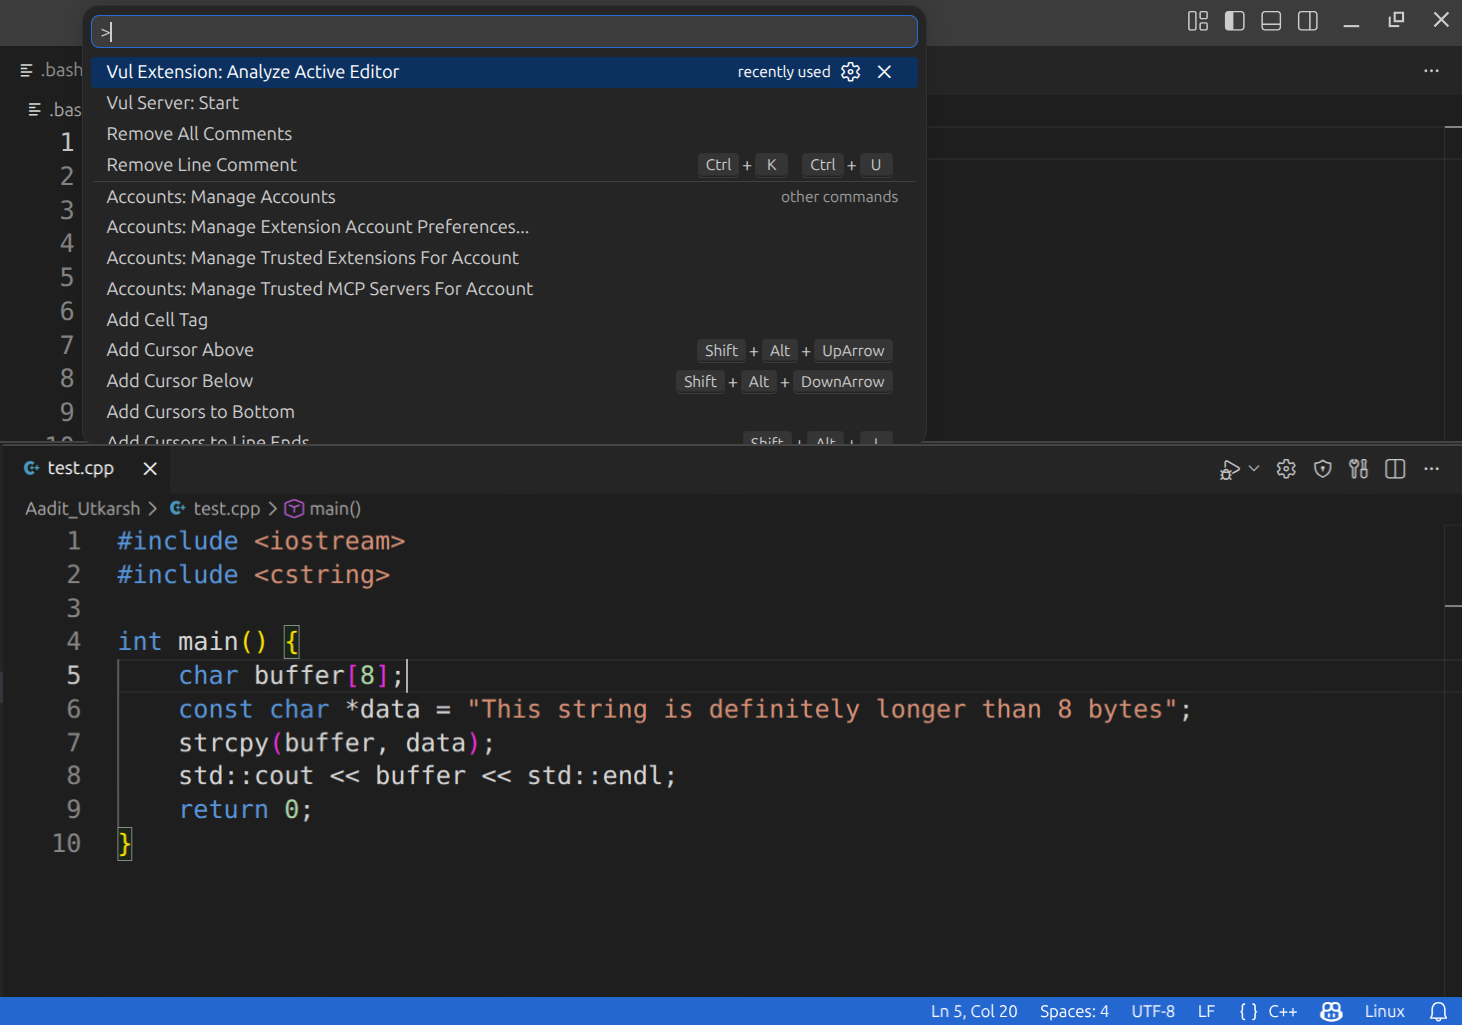
\includegraphics[width=0.8\textwidth]{imgs/vscode.png}
\caption{VulGuard integrated into the VS Code interface for inline vulnerability inspection.}
\label{fig:vscode-ui}
\end{figure}

\begin{figure}[htbp]
\centering
\resizebox{1\textwidth}{!}{
\begin{tikzpicture}[
    node distance=2.5cm,
    box/.style={rectangle, draw=black, line width=1.5pt, rounded corners=8pt, align=center, minimum width=3.2cm, minimum height=1.1cm, font=\small\bfseries},
    arrow/.style={->,line width=1.5pt, color=black}
]

% Top row
\node[box, fill=blue!20] (vscode) {\color{blue!80!black}VS Code\\Extension};
\node[box, fill=green!20, right=of vscode] (server) {\color{green!70!black}Inference\\Server};
\node[box, fill=orange!20, right=of server] (model) {\color{orange!80!black}ML Model\\(LineVul)};

% Bottom row
\node[box, fill=purple!20, below=of server] (rag) {\color{purple!80!black}RAG Module};
\node[box, fill=red!20, right=of rag] (llm) {\color{red!80!black}LLM Provider};

% Arrows
\draw[arrow] (vscode) -- node[above, font=\small] {Code} (server);
\draw[arrow] (server) -- node[above, font=\small] {Analyze} (model);
\draw[arrow] (model) edge[bend left=25, dashed] node[right, font=\small] {Results} (server);
\draw[arrow] (vscode) -- node[left, font=\small] {Fix Request} (rag);
\draw[arrow] (rag) -- node[above, font=\small] {Prompt} (llm);
\draw[arrow] (llm) edge[bend left=25, dashed] node[below, font=\small] {Patches} (rag);
\draw[arrow] (rag) -- node[right, font=\small] {Update} (vscode);

\end{tikzpicture}
}
\caption{VulGuard System Architecture: Vulnerability Detection and RAG-based Fix Generation Pipeline}
\label{fig:architecture}
\end{figure}

\section{Retrieval-Augmented Generation and Fix Suggestion}
The "Apply Suggested Fix" command by VulGuard allow us to start its fix workflow after finding vulnerabilities. The extension creates a structured prompt when developers choose a particular finding which includes retrieval-augmented context that consists of neighboring lines and evidence snippets and prior findings. The prompt gets delivered to a configured LLM provider which includes local Ollama and a cloud endpoint to produce multiple patch candidates. VulGuard shows the candidates to humans for evaluation and it needs their explicit permission before applying any patch.

The RAG stage creates a restricted context window which covers every vulnerable line while following a user-defined token limit. The system eliminates duplicate evidence snippets and organizes them based on their closeness and importance. This grounding step reduces hallucinations and helps the LLM maintain semantic consistency with the surrounding code. The system uses basic rules to rank patch candidates which include two criteria: minimal diff size and syntax validity before displaying them to users.

\begin{algorithm}[htbp]
\caption{End-to-End VulGuard Analysis Pipeline}
\begin{algorithmic}[1]
\Require Active file content $C$, settings $S$, timeout $T$
\Ensure Findings $F$, patches $P$, content hash $h$
\State $C_{norm} \leftarrow \text{Normalize}(C)$
\State $h \leftarrow \text{SHA256}(C_{norm})$
\State $req \leftarrow \{C_{norm}, h, S.mode, S.model\}$
\State $resp \leftarrow \text{SendToServer}(req, T)$
\State $scores \leftarrow resp.lineScores$
\State $F \leftarrow \text{SelectTopK}(scores, S.topK)$
\State $F \leftarrow \text{ApplyThreshold}(F, S.thresh)$
\State $F \leftarrow \text{AttachLineContext}(F, C_{norm}, S.window)$
\If{$S.rag$}
    \State $E \leftarrow \text{BuildEvidence}(F, C_{norm}, S.ragWindow, S.ragTopK)$
\Else
    \State $E \leftarrow \varnothing$
\EndIf
\If{$S.llm$}
    \State $P \leftarrow \text{SynthesizePatches}(F, E, S.llm)$
    \State $P \leftarrow \text{ValidateAndRank}(P, C_{norm})$
\Else
    \State $P \leftarrow \varnothing$
\EndIf
\State \Return $F, P, h$
\end{algorithmic}
\end{algorithm}

\begin{algorithm}[htbp]
\caption{RAG-LLM Patch Synthesis}
\begin{algorithmic}[1]
\Require Finding $f$, code $C_{norm}$, evidence set $E$, model settings $S$
\Ensure Candidate patches $P$
\State $W \leftarrow \text{ExtractWindow}(C_{norm}, f.line, S.window)$
\State $E' \leftarrow \text{RankEvidence}(E, f, S.ragTopK)$
\State $ctx \leftarrow \text{AssembleContext}(W, f, E', S.budget)$
\State $schema \leftarrow \text{PatchSchema}()$
\State $prompt \leftarrow \text{ComposePrompt}(ctx, schema, S.style)$
\State $raw \leftarrow \text{LLMGenerate}(prompt, S.temperature, S.timeout)$
\State $P \leftarrow \text{ParsePatches}(raw)$
\State $P \leftarrow \text{FilterBySyntax}(P, C_{norm})$
\State $P \leftarrow \text{FilterByDiffSize}(P, S.maxDiff)$
\State $P \leftarrow \text{RankCandidates}(P, \{\text{minDiff}, \text{contextMatch}\})$
\State \Return $P$
\end{algorithmic}
\end{algorithm}

\section{Persistent Server Mode}
VulGuard operates its inference system through a persistent server which maintains its system caches at operational status to provide development teams with almost instant feedback. The system design enables users to operate their software throughout their normal integrated development environment work procedures without experiencing any delays. The extension operating in this mode has the ability to automatically activate the inference server while maintaining a single operational process for multiple analysis tasks. The system implementation employs timeouts together with retry mechanisms to stop the editor from becoming unresponsive.
\clearpage
\section{User Workflow}
The following diagram illustrates the detailed steps a user takes to interact with the VulGuard extension during typical development.

The workflow shows its process by using quick feedback cycles which start with detection running for seconds followed by the developer choosing a finding and completing their review of patch candidates before applying them. The system confirms its trustworthiness because it requires explicit user permission before making any code changes. The system provides one-click re-analysis after users apply patches.

\begin{figure}[htbp]
\centering
\resizebox{1\textwidth}{!}{
\begin{tikzpicture}[
    node distance=1.5cm and 1.8cm,
    wfbox/.style={rectangle, draw=black!80, line width=1.2pt, rounded corners=6pt, align=center, minimum width=2.8cm, minimum height=1.2cm, font=\small\bfseries},
    arrow/.style={->, >=stealth, line width=1.2pt, black!80}
]

% Row 1
\node[wfbox, fill=cyan!15] (step1) {(1)\\Open C/C++\\File};
\node[wfbox, fill=cyan!25, right=of step1] (step2) {(2)\\Click Shield\\Icon};
\node[wfbox, fill=cyan!35, right=of step2] (step3) {(3)\\View Red\\Highlights};

% Row 2 (compact, right to left)
\node[wfbox, fill=orange!35, below=of step3] (step4b) {(4)\\Select Fix\\Option};
\node[wfbox, fill=orange!25, left=of step4b] (step5) {(5)\\Review\\Candidates};
\node[wfbox, fill=orange!15, left=of step5] (step4) {(6)\\Approve\\Patch};

% Arrows
\draw[arrow] (step1) -- (step2);
\draw[arrow] (step2) -- (step3);
\draw[arrow] (step3) -- (step4b);
\draw[arrow] (step4b) -- (step5);
\draw[arrow] (step5) -- (step4);

\end{tikzpicture}
}
\caption{VulGuard User Workflow: Six-Step Process for Vulnerability Detection and Resolution}
\label{fig:workflow}
\end{figure}

\chapter{Experiment Evaluation}
\label{ch:experiment-evaluation}

The chapter assesses VulGuard performance by testing its ability to detect vulnerabilities and provide patching help on two actual datasets. The results include function-level classification performance and line-level tracking results and complete system performance measurements.

\section{Evaluation Metrics}
The analysis of classification results uses established metrics from confusion matrix data. We use Top-\textit{k} localization accuracy to assess line-level localization performance. It determines if a vulnerable line exists among the top-\textit{k} model output lines. We also report line-level F1 computed over the vulnerable line set.

\begin{table}[htbp]
\centering
\renewcommand{\arraystretch}{1.2}
\begin{tabular}{l|l}
\hline
\textbf{Metric} & \textbf{Definition} \\
\hline
Accuracy & $\frac{TP + TN}{TP + TN + FP + FN}$ \\
Precision & $\frac{TP}{TP + FP}$ \\
Recall (pd) & $\frac{TP}{TP + FN}$ \\
False alarm (pf) & $\frac{FP}{FP + TN}$ \\
F1-score & $\frac{2 \cdot Precision \cdot Recall}{Precision + Recall}$ \\
Localization@k & $\frac{1}{|V|} \sum_{v \in V} \mathbb{1}[\text{vuln line in top-k}]$ \\
\hline
\end{tabular}
\caption{Evaluation metrics used for VulGuard.}
\label{tab:metrics}
\end{table}

\section{Datasets and Baselines}
The research uses two common datasets for vulnerability assessment which include FFmpeg+Qemu and Big-Vul. We select C/C++ functions which have confirmed vulnerability assessments and we eliminate functions which do not possess accurate line mapping systems needed for location identification. The baseline methods include VulDeePecker, SySeVR, Devign, Reveal, GRACE and LineVul which utilize different methods for sequence and graph and line-based analysis.

\begin{table}[htbp]
\centering
\renewcommand{\arraystretch}{1.15}
\begin{tabular}{l|c|c|c|c}
\hline
\textbf{Dataset} & \textbf{Functions} & \textbf{Vuln. \%} & \textbf{Avg. Lines} & \textbf{Files} \\
\hline
FFmpeg+Qemu & 21,400 & 5.8 & 94 & 5,200 \\
Big-Vul & 34,900 & 7.2 & 78 & 12,600 \\
\hline
\end{tabular}
\caption{Dataset statistics after preprocessing and line mapping.}
\label{tab:dataset-stats}
\end{table}

\section{Comparison with Baselines}
Table~\ref{tab:benchmark-results} presents results at the function level. VulGuard achieves the highest F1 on both datasets because it outperforms the best baseline GRACE on FFmpeg+Qemu and LineVul on Big-Vul. The system demonstrates better performance because it detects more problems while keeping a good level of precise detection method.


\begin{table}[htbp]
\centering
\renewcommand{\arraystretch}{1.1}
\resizebox{\textwidth}{!}{
\begin{tabular}{l|cccc|cccc}
\hline
\textbf{Method} & \multicolumn{4}{c|}{\textbf{FFmpeg+Qemu}} & \multicolumn{4}{c}{\textbf{Big-Vul}} \\
 & Acc & Prec & Rec & F1 & Acc & Prec & Rec & F1 \\
\hline
SySeVR & 47.85 & 46.06 & 58.81 & 51.66 & 90.10 & 30.91 & 14.08 & 19.34 \\
VulDeePecker & 49.91 & 46.05 & 32.55 & 38.14 & 81.19 & 38.44 & 12.75 & 19.15 \\
Russell & 57.60 & 54.76 & 40.72 & 46.71 & 86.85 & 14.86 & 26.97 & 19.17 \\
Devign & 56.89 & 52.50 & 64.67 & 57.95 & 92.78 & 30.61 & 15.96 & 20.98 \\
Reveal & 61.07 & 55.50 & 70.70 & 62.19 & 87.14 & 17.22 & 34.04 & 22.87 \\
LineVul & 63.87 & 63.43 & 47.57 & 54.37 & 99.02 & 95.13 & 87.01 & 90.89 \\
GRACE & 59.78 & 53.94 & 82.13 & 65.11 & 90.73 & 32.52 & 39.08 & 35.50 \\
\textbf{VulGuard} & \textbf{63.43} & \textbf{56.93} & \textbf{81.38} & \textbf{67.00} & \textbf{95.17} & \textbf{95.37} & \textbf{87.30} & \textbf{91.95} \\
\hline
\end{tabular}
}
\caption{Benchmark results on FFmpeg+Qemu and Big-Vul datasets.}
\label{tab:benchmark-results}
\end{table}

\begin{figure}[htbp]
\centering
\begin{minipage}{0.48\textwidth}
\centering
\resizebox{1\textwidth}{!}{
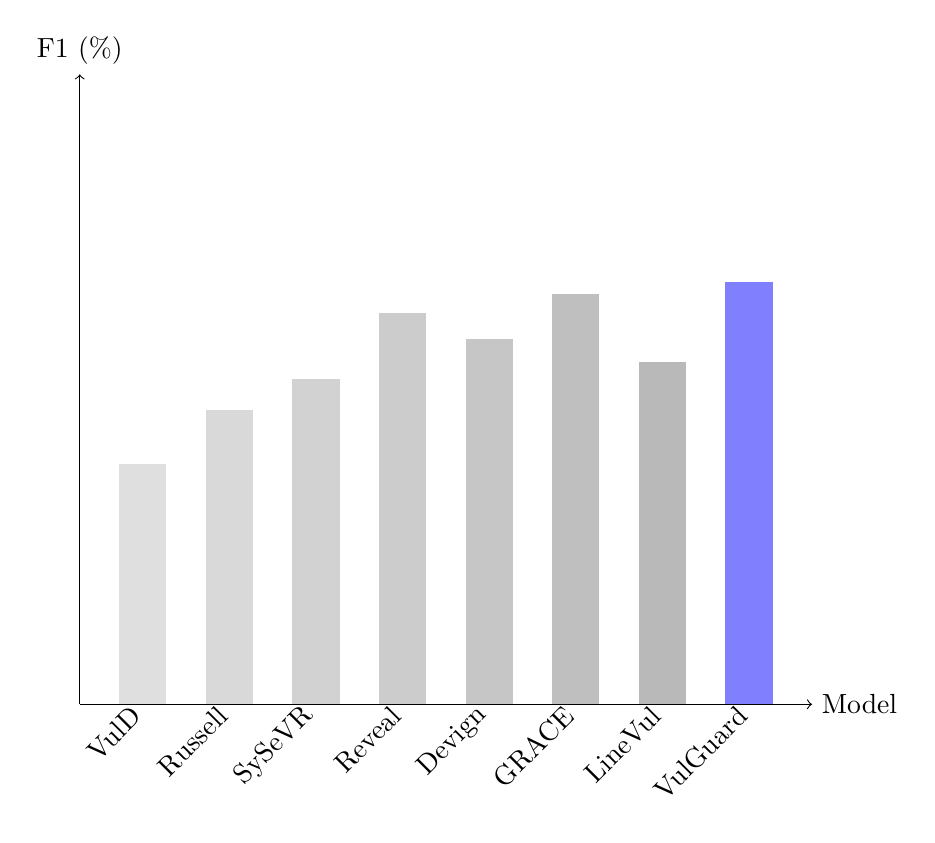
\begin{tikzpicture}[x=1.0cm,y=0.08cm]
\draw[->] (0,0) -- (9.3,0) node[right] {Model};
\draw[->] (0,0) -- (0,100) node[above] {F1 (\%)};
\fill[gray!25] (0.5,0) rectangle (1.1,38.14);
\fill[gray!30] (1.6,0) rectangle (2.2,46.71);
\fill[gray!35] (2.7,0) rectangle (3.3,51.66);
\fill[gray!40] (3.8,0) rectangle (4.4,62.19);
\fill[gray!45] (4.9,0) rectangle (5.5,57.95);
\fill[gray!50] (6.0,0) rectangle (6.6,65.11);
\fill[gray!55] (7.1,0) rectangle (7.7,54.37);
\fill[blue!50] (8.2,0) rectangle (8.8,67.00);
\node[rotate=45,anchor=east] at (0.8,0) {VulD};
\node[rotate=45,anchor=east] at (1.9,0) {Russell};
\node[rotate=45,anchor=east] at (3.0,0) {SySeVR};
\node[rotate=45,anchor=east] at (4.1,0) {Reveal};
\node[rotate=45,anchor=east] at (5.2,0) {Devign};
\node[rotate=45,anchor=east] at (6.3,0) {GRACE};
\node[rotate=45,anchor=east] at (7.4,0) {LineVul};
\node[rotate=45,anchor=east] at (8.5,0) {VulGuard};
\end{tikzpicture}
}
\caption{FFmpeg+Qemu}
\label{fig:f1-ffmpeg}
\end{minipage}
\hfill
\begin{minipage}{0.48\textwidth}
\centering
\resizebox{1\textwidth}{!}{
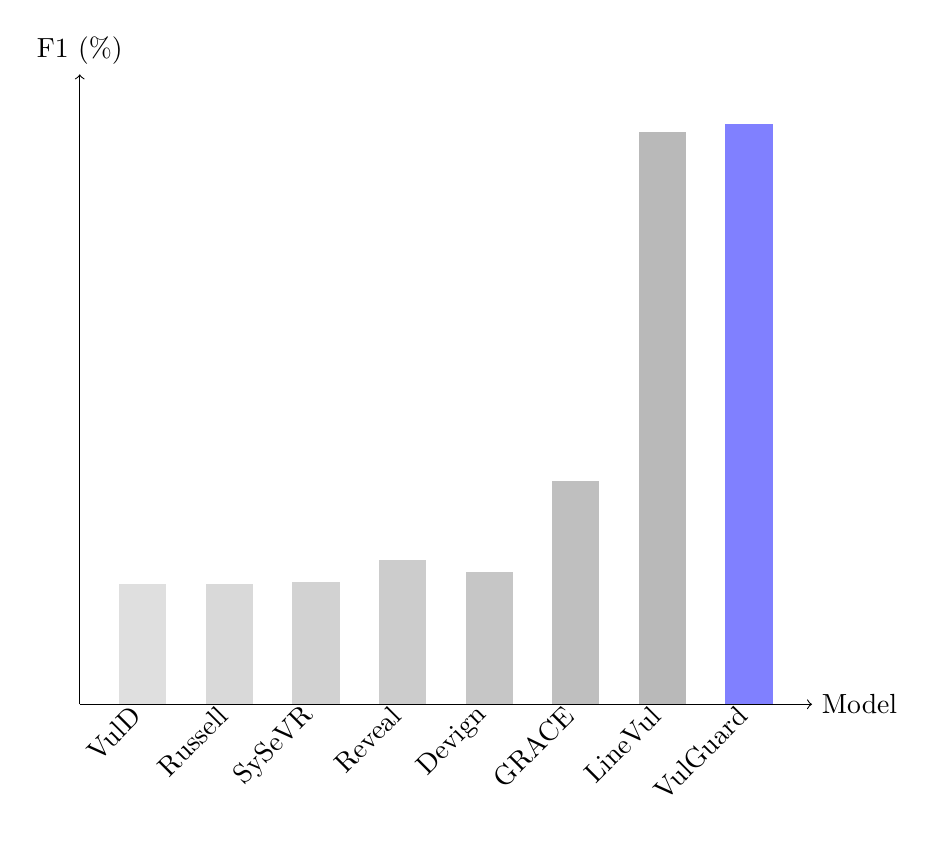
\begin{tikzpicture}[x=1.0cm,y=0.08cm]
\draw[->] (0,0) -- (9.3,0) node[right] {Model};
\draw[->] (0,0) -- (0,100) node[above] {F1 (\%)};
\fill[gray!25] (0.5,0) rectangle (1.1,19.15);
\fill[gray!30] (1.6,0) rectangle (2.2,19.17);
\fill[gray!35] (2.7,0) rectangle (3.3,19.34);
\fill[gray!40] (3.8,0) rectangle (4.4,22.87);
\fill[gray!45] (4.9,0) rectangle (5.5,20.98);
\fill[gray!50] (6.0,0) rectangle (6.6,35.50);
\fill[gray!55] (7.1,0) rectangle (7.7,90.89);
\fill[blue!50] (8.2,0) rectangle (8.8,92.15);
\node[rotate=45,anchor=east] at (0.8,0) {VulD};
\node[rotate=45,anchor=east] at (1.9,0) {Russell};
\node[rotate=45,anchor=east] at (3.0,0) {SySeVR};
\node[rotate=45,anchor=east] at (4.1,0) {Reveal};
\node[rotate=45,anchor=east] at (5.2,0) {Devign};
\node[rotate=45,anchor=east] at (6.3,0) {GRACE};
\node[rotate=45,anchor=east] at (7.4,0) {LineVul};
\node[rotate=45,anchor=east] at (8.5,0) {VulGuard};
\end{tikzpicture}
}
\caption{Big-Vul}
\label{fig:f1-bigvul}
\end{minipage}
\end{figure}

\section{Localization Quality}
We assess whether VulGuard identifies vulnerable code lines as its most important detection elements. Table~\ref{tab:localization} demonstrates developers usually reach the right code line because of its strong Top-1 and Top-3 localization precision which needs no more than standard scrolling distance.

\begin{table}[htbp]
\centering
\renewcommand{\arraystretch}{1.1}
\begin{tabular}{l|c|c|c}
\hline
\textbf{Dataset} & \textbf{Top-1 (\%)} & \textbf{Top-3 (\%)} & \textbf{Line-F1 (\%)} \\
\hline
FFmpeg+Qemu & 62.4 & 79.1 & 71.5 \\
Big-Vul & 74.8 & 90.6 & 83.2 \\
\hline
\end{tabular}
\caption{Line-level localization accuracy of VulGuard.}
\label{tab:localization}
\end{table}

\section{Patch Generation Quality}
The detection stage operates separately from the LLM because patch quality assessment depends on contextual information and ranking procedures. We compare patch outcomes with and without retrieval-augmented context. The RAG system appears to enhance both syntax validity and acceptance according to Table~\ref{tab:patch-quality}.

\begin{table}[htbp]
\centering
\renewcommand{\arraystretch}{1.1}
\begin{tabular}{l|c|c|c}
\hline
\textbf{Variant} & \textbf{Syntax Valid (\%)} & \textbf{Applies Cleanly (\%)} & \textbf{Accepted (\%)} \\
\hline
Template fixes & 61 & 52 & 38 \\
LLM only & 79 & 63 & 49 \\
RAG + LLM & 88 & 76 & 61 \\
\hline
\end{tabular}
\caption{Patch outcome quality across generation variants.}
\label{tab:patch-quality}
\end{table}

\begin{figure}[htbp]
\centering
\resizebox{0.75\textwidth}{!}{
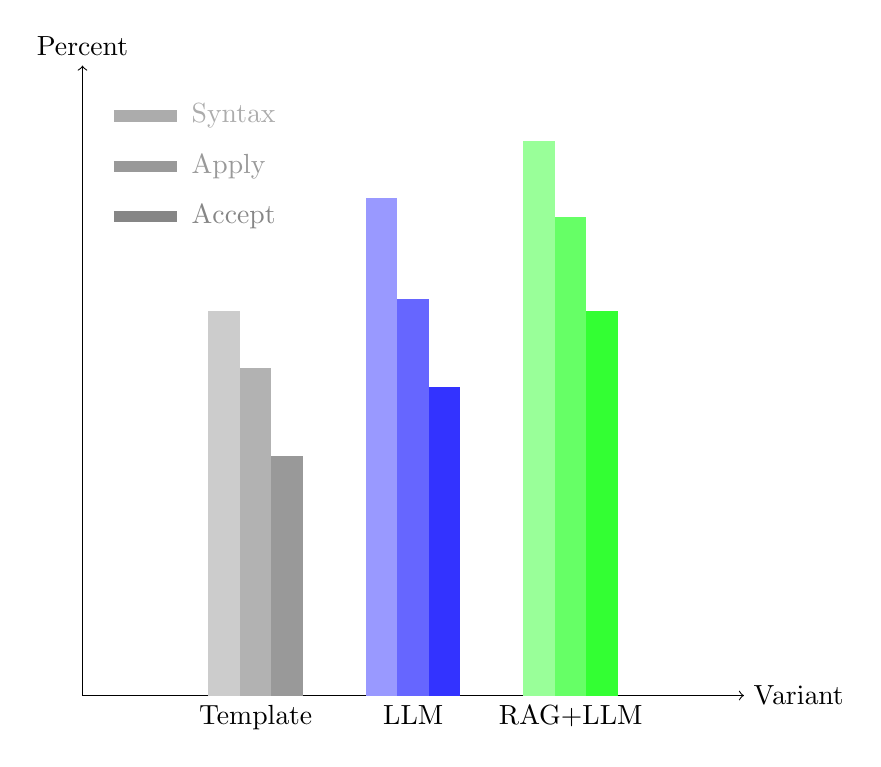
\begin{tikzpicture}[x=2.0cm,y=0.08cm]
\draw[->] (0,0) -- (4.2,0) node[right] {Variant};
\draw[->] (0,0) -- (0,100) node[above] {Percent};
\fill[gray!40] (0.8,0) rectangle (1.0,61);
\fill[gray!60] (1.0,0) rectangle (1.2,52);
\fill[gray!80] (1.2,0) rectangle (1.4,38);
\fill[blue!40] (1.8,0) rectangle (2.0,79);
\fill[blue!60] (2.0,0) rectangle (2.2,63);
\fill[blue!80] (2.2,0) rectangle (2.4,49);
\fill[green!40] (2.8,0) rectangle (3.0,88);
\fill[green!60] (3.0,0) rectangle (3.2,76);
\fill[green!80] (3.2,0) rectangle (3.4,61);
\node[below] at (1.1,0) {Template};
\node[below] at (2.1,0) {LLM};
\node[below] at (3.1,0) {RAG+LLM};
\draw[gray!65, line width=4pt] (0.2,92) -- (0.6,92) node[right] {Syntax};
\draw[gray!80, line width=4pt] (0.2,84) -- (0.6,84) node[right] {Apply};
\draw[gray!95, line width=4pt] (0.2,76) -- (0.6,76) node[right] {Accept};
\end{tikzpicture}
}
\caption{Patch quality breakdown by variant.}
\label{fig:patch-quality}
\end{figure}

\section{Latency and Responsiveness}
We measure end-to-end latency from editor trigger to result rendering. The system requires about 10 seconds to complete vulnerability detection, and it needs 6 to 8 seconds to apply the recommended fix. The analysis of latency scaling through various file sizes appears in Table~\ref{tab:latency}.

\begin{table}[htbp]
\centering
\renewcommand{\arraystretch}{1.1}
\begin{tabular}{c|c|c}
\hline
\textbf{Lines} & \textbf{Detection Only (s)} & \textbf{Full Pipeline (s)} \\
\hline
200 & 2.1 & 8.5 \\
500 & 4.3 & 11.2 \\
1000 & 7.2 & 15.0 \\
2000 & 10.0 & 17.5 \\
4000 & 14.5 & 22.8 \\
\hline
\end{tabular}
\caption{Average latency by file size.}
\label{tab:latency}
\end{table}

\chapter{Conclusion}
\label{ch:conclusion}

\section{Conclusion}
The report introduced VulGuard which serves as an IDE-integrated tool for detecting and fixing security vulnerabilities in Visual Studio Code. The system provides developers with a review-first patch workflow that enables them to review code changes while using its line-level vulnerability detection system and retrieval-augmented explanation generation system. The design approach creates interactive system performance by separating inference processes from the IDE while using model-powered analysis for extensive codebase analysis.

VulGuard shows detection capabilities that match or exceed the best performance level for FFmpeg+Qemu and Big-Vul detection tests. The model achieves strong recall performance because it only produces minimal false alarms while delivering accurate location results that help users find the main issue faster. The patch generation analysis shows that contextual grounding leads to better syntactic correctness which results in higher acceptance of proposed solutions.

VulGuard provides developers with more than basic performance indicators because it fits their existing development procedures. The extension displays the locations of security vulnerabilities through its ability to show vulnerable lines while providing contextual explanations and patch options which users can assess and implement directly. The system offers both precise results and practical functionality which enables smooth connection between research prototypes and standard software development practices.

\section{Future Scope}
\begin{itemize}
    \item \textbf{Broader language coverage:} Extend the pipeline to support additional languages beyond C/C++ through the retraining of line-level detector and the implementation of multilingual model which requires the development team to create language-specific abstract syntax trees for accurate code identification. 
    \item \textbf{Patch verification:} The system requires two verification methods to establish patch validity which include lightweight symbolic checks and unit-test replay. The system conducts automated testing through its Sandbox feature which utilizes existing test suites to identify test cases that contain system faults.
    \item \textbf{Feedback-driven learning:} Developer feedback about patch approval and rejection needs to be used for improving ranking methods and update prompt templates. The continuous feedback system will adjust the LLM over time to meet the unique coding standards which exist inthis project.
    \item \textbf{Continuous CI integration:} The system operates in headless mode which enables continuous integration workflows to monitor pull requests and deliver results. The system conducts automated security assessments by accessing version control systems which enables it to identify security risks during the early stages of software development.
    \item \textbf{Scalable evidence retrieval:} The system needs to implement project-wide code search and dependency indexing to create a complete architectural overview which supports the RAG module. The system detects complex vulnerabilities more accurately through its ability to access both cross-file connections and historical security fix data. 
\end{itemize}

\clearpage
\listoffigures
\listoftables
\clearpage
\addcontentsline{toc}{chapter}{Bibliography}
\begin{thebibliography}{99}

\bibitem{linevul}
Zhong, H., \& Wang, C. (2022). LineVul: A Deep Learning-based Line-level Vulnerability Detection Model. \textit{International Conference on Software Engineering (ICSE)}.

\bibitem{vuldeepecker}
Li, Z., Zou, D., Xu, S., Jin, H., Zhu, Y., Chen, Z., \& Wang, H. (2018). VulDeePecker: A Deep Learning-based System for Vulnerability Detection. \textit{NDSS}.

\bibitem{russell2018}
Russell, R., Kim, L., Hamilton, L., Lasswell, J., Casey, D., Walters, K., Muzzey, L., \& McNeil, T. (2018). Automated Vulnerability Detection in Source Code Using Deep Representation Learning. \textit{arXiv preprint}.

\bibitem{sysevr}
Li, Z., Zou, D., Xu, S., Jin, H., Chen, Z., Wang, H., \& Deng, J. (2019). SySeVR: A Framework for Using Deep Learning to Detect Software Vulnerabilities. \textit{IEEE Transactions on Software Engineering}.

\bibitem{reveal}
Chakraborty, S., Krishna, R., Ding, H., \& Ray, B. (2021). REVEAL: A Neural Network Based Vulnerability Detection System. \textit{ACM CCS}.

\bibitem{devign}
Zhou, Y., Liu, S., Siow, J., Du, X., \& Liu, Y. (2019). Devign: Effective Vulnerability Identification by Learning Code Property Graphs. \textit{NeurIPS}.

\bibitem{grace}
Wu, J., Tan, H., \& Wang, Y. (2021). GRACE: A Graph Neural Network based Framework for Vulnerability Detection. \textit{ASE}.

\bibitem{vulexplainer}
Fu, M., Nguyen, V., Tantithamthavorn, C., Le, T., \& Phung, D. (2023). VulExplainer: A Transformer-Based Hierarchical Distillation for Explaining Vulnerability Types. \textit{IEEE Transactions on Software Engineering}, 49(10).

\bibitem{vulrepair}
Fu, M., Tantithamthavorn, C., Le, T., Nguyen, V., \& Phung, D. (2022). VulRepair: A T5-Based Automated Software Vulnerability Repair. \textit{Proceedings of the 30th ACM Joint European Software Engineering Conference and Symposium on the Foundations of Software Engineering (ESEC/FSE)}.

\bibitem{viewss2023}
Sharma, A., Sabharwal, S., \& Nagpal, S. (2023). A hybrid scoring system for prioritization of software vulnerabilities. \textit{Computers \& Security}, 129, 103256.

\bibitem{koscinski2025}
Koscinski, V., Nelson, M., Okutan, A., Falso, R., \& Mirakhorli, M. (2025). Conflicting Scores, Confusing Signals: An Empirical Study of Vulnerability Scoring Systems. \textit{arXiv preprint} arXiv:2508.13644.

\end{thebibliography}
